\input TinLatex.tex
% \usepackage{hyperref}
% \hypersetup{colorlinks,linkcolor={blue},citecolor={blue},urlcolor={red}}  
\setlength{\paperheight}{11in}
\setlength{\paperwidth}{8.5in}
% \bibliographystyle{IEEEtranS} % sorted IEEE style
% \bibliographystyle{IEEEtran} % Đặt kiểu trích dẫn là IEEEtran
\usepackage{multirow}
\usepackage{enumitem}
% \usepackage[ruled,linesnumbered]{algorithm2e}
	% \SetAlgorithmName{Algorithm}{algorithm}{}
\usepackage{amsmath}

\NewDocumentCommand{\MYref}{O{black}mo}{%
  \begingroup
  \hypersetup{linkcolor=#1}%
  \ref{#2}%
  \IfValueT{#3}{%
    \color{#1}{#3}%
  }%
  \endgroup
}% %NEW COMMAND ALTERNATIVE TO REF

\newcommand\MYreforig[3][black]{\begingroup\hypersetup{linkcolor=#1}\ref{#3}{\color{#1}{#3}}\endgroup}% 

\usepackage{caption} 
\usepackage{cleveref}
\usepackage{color,soul}
\usepackage{pagecolor}
\usepackage{amsthm}
\usepackage{amsfonts}
\usepackage{amssymb}
\usepackage{amsmath}
\newtheorem{assumption}{Assumption}
\newtheorem{remark}{Remark}
\newtheorem{lemma}{Lemma}
\newtheorem{theorem}{Theorem}
\newtheorem{definition}{Definition}
% \newtheorem{proof}{Proof}
\newtheorem{example}{Example}
\usepackage{orcidlink}
\usepackage{algpseudocode}
\usepackage{indentfirst}
\usepackage{algorithm}
\usepackage{algpseudocode}




% \renewcommand\hl{}
\begin{document}
\makeatletter	   % `@' is now a normal "letter' for LaTeX
\setcounter{page}{1}
\renewcommand{\ps@plain}{%
	\renewcommand{\@oddhead}{\hfill\begin{tabular}{r}
			\small{\emph{Journal of Computer Science and Cybernetics, V.40, N.3 (2025), 1-}} \\
			\footnotesize{DOI: 10.15625/1813-9663/19558}
		\end{tabular}
	}
	
	\renewcommand{\@evenhead}{\@oddhead}
	\renewcommand{\@oddfoot}{
		%\small\hfill{\hskip7.1cm \copyright\ 2024 Vietnam  Academy of Science \& Technology}
		\renewcommand{\@evenfoot}{\@oddfoot}
	}
}

%Lenh duoi thay doi do dai cua duong ngang
%\usepackage[flushmargin]{footmisc} - PHẢI MỞ LỆNH NÀY
\def\footnoterule{\kern-3\p@
	\hrule \@width 1.32in \kern 2.6\p@} % the \hrule is .4pt high
%Thay doi indent cua footnote
%\renewcommand{\footnotesep}{2cm}
% \renewcommand{\footnotemargin}{0em}
\newcommand{\fn}[1]{\footnotetext{\hspace{-6mm}#1}}
\setlength{\skip\footins}{8mm}

\makeatother   % `@' is restored as a "non-letter" character 
    
%%%%%%%%%%%%%%%%%%%%%%%%
%Title & Authors
%%%%%%%%%%%%%%%%%%%%%%%%

%=========================================================================
\title{AUTHOR GUIDELINES FOR JCC SUBMISSION}
\subtitle{SUBTITLE}
\author{
	{\cn AUTHOR NAME(S) 1, AUTHOR NAME(S) 2}
	\vskip.5cm
	{
    \it $^1$Institute of Information Technology, Vietnam Academy of Science and Technology, \\ 18 Hoang Quoc Viet Street, Cau Giay District, Ha Noi, Viet Nam\\
        \it $^2$Thai Nguyen University of Information and Communication Technology, Z115 Street, Quyet Thang Ward, Thai Nguyen City, Viet Nam\\
\fn{*Corresponding author.}
\fn{\hspace{1.7mm}{\it E-mail addresses}:
\href{mailto:anonymous@ioit.ac.vn}{anonymous@ioit.ac.vn} (AUTHOR NAME(S) 1); 
\href{mailto:anonymous@ioit.ac.vn}{anonymous@tnu.edu.vn} (AUTHOR NAME(S) 2).
}}}
\maketitle
\renewcommand\refname{\normalsize \centerline{ REFERENCES}}
% Set to use the "plain" pagestyle
\pagestyle{plain}
\pagestyle{myheadings}
\markboth{\footnotesize \chu \uppercase{AUTHOR NAME(S) 1} {\it et al.}}
{\footnotesize  \chu \uppercase{Attribute Reduction Based on Rough Set Theory }}% Maximun 8 words 
{	\vspace{-.4cm}
	%\hspace{13.25cm}{\includegraphics[scale=.2]{crosscheck.pdf}}%\vspace{-.5cm}
	\hspace{13.04cm}{\includegraphics[scale=.05]{cross_check.PNG}
	}
}
%=========================================================================

{\cn
%=========================================================================
\begin{abstract}{The abstract should be fully justified and formatted in a one-column layout, positioned below the author and affiliation information. Use the word “Abstract” as the title, in 12-point Times, boldface type, with initial capitalization. The abstract should be written in 11-point, single-spaced text. It must summarize the contents of the paper, including its context, main content, and conclusions, in fewer than 200 words.}
\vn
\end{abstract}
\textbf{Keyword.} We would like to encourage you to list your keywords within the abstract section. Enter key words or phrases in lower case alphabetical order, separated by commas.
}


%%%%%%%%%%%%%%%%%%%%%%%%
%Main text
%%%%%%%%%%%%%%%%%%%%%%%%

%=========================================================================
\section{INTRODUCTION}

Please follow the steps outlined below when submitting your manuscript to the Journal of Computer Science and Cybernetics. This style guide now has several important modifications, so all authors should read this new version.
\subsection{Language}
Contributions to Journal of Computer Science and Cybernetics are to be in American English. Authors are encouraged to have their contribution checked for grammar. American spelling should be used. Abbreviations are allowed but should be spelt out in full when first used. Integers ten and below are to be spelt out. Italicize foreign language phrases (e.g. Latin, French). Upon acceptance, authors are required to submit their data source file including postscript files for figures.
\subsection{Dual submission}
By submitting a manuscript to JCC, the authors guarantee that it has not been previously published or accepted for publication in substantially similar form in an archival peer-reviewed forum. Furthermore, no paper which contains significant overlap with the contributions of this paper is neither under review at the moment of submission nor will be submitted during the JCC review period to \textbf{any of the following}: another conference, a workshop, or a journal. The authors also attest that they did not submit substantially similar submissions to JCC. Violation of any of these conditions will lead to rejection. If you are not sure about the extent of overlap, you may upload a copy of the paper in question as supplementary material. Note that a Technical Report (departmental, arXiv.org, etc.) that is put up without any form of direct peer-review is \textbf{NOT} considered a publication. Likewise, mention of the work under review in a presentation is \textbf{NOT} considered a violation.

If there are any papers that may appear to the reviewers to violate this condition, then it is your responsibility to (1) cite these papers, (2) argue in the body of your paper why your JCC paper is nontrivially different from these concurrent submissions, and (3) include anonymized versions of those papers in the supplemental material.
\subsection{Paper length}
The minimum paper length is 8 pages. The maximum lengths of a research paper and a survey paper are respectively 15 pages and 20 pages. Overlength and underlength papers will simply not be reviewed. This includes papers where the margins and formatting are deemed to have been significantly altered from those laid down by this style guide.
%=========================================================================
\subsection{Equations}

Displayed equations should be numbered consecutively in each section, with the number set flush right and enclosed in parentheses
\begin{equation}
a^2 = b^2+c^2.
\end{equation}

Please number all of your sections and displayed equations. It is important for readers to be able to refer to any particular equation. Just because you did not refer to it in the text does not mean some future reader might not need to refer to it. It is cumbersome to have to use circumlocutions like “the second equation from the top of page 3 column 1”. Equations should be referred to in abbreviated form, e.g. “Eq. 1” or “2”. In multiple-line equations, the number should be given on the last line. Displayed equations are to be centered on the page width. Standard English letters like $x$ are to appear as $x$ (italicized) in the text if they are used as mathematical symbols. Punctuation marks are used at the end of equations as if they appeared directly in the text. References to equation labels are in black.
%-------------------------------------------------------------------------
\subsection{Miscellaneous}

When citing a multi-author paper, you may save space by using “et alia”, shortened to “et al.” (not “et. al.” as “et” is a complete word.) However, use it only when there are three or more authors.  Thus, the following is correct: “Frobnication has been trendy lately. It was introduced by Alpher \cite{b1}, and subsequently developed by Alpher and Fotheringham-Smythe \cite{b2}, and Alpher et al. \cite{b3}.”

This is incorrect: “… subsequently developed by Alpher et al. \cite{b2} …” because reference \cite{b2} has just two authors.

For this citation style, keep multiple citations in numerical (not chronological) order, so prefer \cite{b1, b2, b3} to \cite{b2, b1, b3}. 



%\begin{figure*}
%\begin{center}
%\fbox{\rule{0pt}{2in} \rule{.9\linewidth}{0pt}}
%\end{center}
%   \caption{\small Example of a short caption, which should be centered.}
%\label{fig:short}
%\end{figure*}
%

%=========================================================================
\section{FORMATTING YOUR PAPER}

All text must be in a one-column format. The main title (on the first page) should begin 1.0 inch (2.54 cm) from the top edge of the page. The second and following pages should begin 1.0 inch (2.54 cm) from the top edge. On all pages, the bottom margin should be 1-1/8 inches (2.86 cm) from the bottom edge of the page for $8.5 \times 11$-inch paper; for A4 paper, approximately 1-5/8 inches (4.13 cm) from the bottom edge of the page.

%-------------------------------------------------------------------------
\subsection{Margins and page numbering}

All printed material, including text, illustrations, and charts, must be kept within a print area 6-7/8 inches (17.5 cm) wide by 8-7/8 inches (22.54 cm) high.

%-------------------------------------------------------------------------
\subsection{Type-style and fonts}

Wherever Times is specified, Times Roman may also be used. If neither is available on your word processor, please use the font closest in appearance to Times to which you have access.

MAIN TITLE is centered and positioned 1-3/8 inches (3.49 cm) from the top edge of the first page. The title should be in Calibri 14-point, boldface capitalized type. A subtitle may be optionally included. Leave a blank line after the title.

AUTHOR NAME(s) and AFFILIATION(s) are to be centered beneath the title and printed in Times 11-point, non-boldface type. This information is to be followed by one blank line.

The ABSTRACT and MAIN TEXT are to be in a one-column format.

MAIN TEXT is to be typeset in 11-point Times, single-spaced. Do NOT use double-spacing. All paragraphs should be indented 1 pica (approx. 1/6 inch or 0.422 cm). Make sure your text is fully justified---that is, flush left and flush right. Please do not place any additional blank lines between paragraphs.

MAJOR HEADINGS. (For example \textbf{1. Introduction}) should be Times 12-point boldface, capitalized, flush left, with one blank line before, and one blank line after.

SUB HEADINGS (For example, \textbf{1.1. Database elements}) should be Times 11-point boldface, initially capitalized, flush left, with one blank line before, and one after. If you require a third-order heading (we discourage it), use 10-point Times, boldface, initially capitalized, flush left, preceded by one blank line, followed by a period and your text on the same line.

If you know the Digital Object Identifier (DOI) number of your article, place it at the header of page 1 using Times 9-point type.


%-------------------------------------------------------------------------
\subsection{Footnotes}

Please use footnotes\footnote{This is what a footnote looks like.  It often distracts the reader from the main flow of the argument.} sparingly. Indeed, try to avoid footnotes altogether and include necessary peripheral observations in the text (within parentheses, if you prefer, as in this sentence).  If you wish to use a footnote, place it at the bottom of the column on the page on which it is referenced. Use Times 9-point type, single-spaced. Footnotes in the body text should be numbered sequentially in superscript lowercase Roman letters.  

%-------------------------------------------------------------------------
\subsection{Program code}

Fragments of computer programs and algorithm descriptions in the text are typically set in a typewriter font, such as \eg, CMTT10 or Courier. Use the same font size for keywords, variables, and other elements as in the main text. Do not use a smaller typeface to force program fragments and algorithms to fit within the document’s predefined margins.

\noindent
{\it Example of a Computer Program}
\begin{verbatim}
program Inflation (Output)
  {Assuming annual inflation rates of 7%, 8%, and 10%,...
   years};
   const
     MaxYears = 10;
   var
     Year: 0..MaxYears;
     Factor1, Factor2, Factor3: Real;
   begin
     Year := 0;
     Factor1 := 1.0; Factor2 := 1.0; Factor3 := 1.0;
     WriteLn('Year  7% 8% 10%'); WriteLn;
     repeat
       Year := Year + 1;
       Factor1 := Factor1 * 1.07;
       Factor2 := Factor2 * 1.08;
       Factor3 := Factor3 * 1.10;
       WriteLn(Year:5,Factor1:7:3,Factor2:7:3,Factor3:7:3)
     until Year = MaxYears
end.
\end{verbatim}
%
\noindent
{\small (Example from Jensen K., Wirth N. (1991) Pascal user manual and
report. Springer, New York)}

%-------------------------------------------------------------------------
% \begin{algorithm}[H]
% \caption{Parallel Algorithm}
% \textbf{Input:} $s$ is a vertex of the polyhedral surface. \\
% \textbf{Output:} A funnel tree that contains the shortest paths from $s$ to all vertices of the surface.
% \begin{algorithmic}[1]
% \State $root := s$
% \For {each edge $[p, q]$ opposite to $s$}
%     \State Insert $F_{p,q,S}$ as root's children
% \EndFor
% \For {$k = 1, 2,\ldots, n $} \Comment{$n$ is the number of faces}\\
%     \hspace{0.25cm}\textbf{Parallel for} each funnel (node) $F_{p,q,S}$ at the $k^{th}$ level \textbf{do}
%         \hspace{1cm}\State Find direct destination $v$ of $F_{p,q,S}$ such that $\beta_v < 180^\circ$ \Comment{$\beta_v$ is  computed by the formula (4) in \cite{19}}
%         \hspace{1cm}\If {such vertex does not exist}
%             \hspace{1cm}\State $F_{p,q,S}$ has no children, \textbf{Continue}
%         \hspace{1cm}\Else
%             \hspace{1cm}\State Let $S' := S \cup \triangle pqv$
%             \hspace{1cm}\If {$\angle psv < \angle psw$}
%                 \hspace{1cm}\State $F_{p,q,S}$ has 2 children $F_{p,v,S'}, F_{v,q,S'}$. Insert them into the funnel tree and mark $\angle pvq$
%             \hspace{1cm}\Else
%                 \hspace{1cm}\State $F_{p,q,S}$ has one child $F_{p,v,S'}$. Insert it into the funnel tree
%             \hspace{1cm}\EndIf
%         \hspace{1cm}\EndIf\\
%     \hspace{0.25cm}\textbf{end for}
%     \For {each funnel $F_{p,q,S}$ at the $k^{th}$ level}
%         \If {$\angle pvq$ is previously marked by another funnel called $F_{p,q,S_1}$}
%             \State Call \textsc{Clip\_off\_Funnels}($\triangle pqv, S, S_1$) \Comment{ See procedure \textsc{Clip\_off\_Funnels} in \cite{19}}
%         \EndIf
%     \EndFor
%     \If {$(k+1)^{th}$ level has no nodes}
%         \State \textbf{Break}
%     \EndIf
% \EndFor
% \end{algorithmic}
% \end{algorithm}


\begin{algorithm}[H]
\caption{Parallel Algorithm}
\textbf{Input:} $s$ is a vertex of the polyhedral surface. \\
\textbf{Output:} A funnel tree that contains the shortest paths from $s$ to all vertices of the surface.
\begin{algorithmic}[1]
\State $root \gets s$
\For {each edge $[p, q]$ opposite to $s$}
    \State Insert $F_{p,q,S}$ as root's children
\EndFor
\For {$k = 1, 2, \ldots, n$} \Comment{$n$ is the number of faces}
    \ForAll {funnels (nodes) $F_{p,q,S}$ at the $k^{th}$ level \textbf{in parallel}}
        \State Find direct destination $v$ of $F_{p,q,S}$ such that $\beta_v < 180^\circ$ \Comment{$\beta_v$ is computed by the formula (4) in \cite{19}}
        \If {such vertex does not exist}
            \State $F_{p,q,S}$ has no children
            \State \textbf{Continue}
        \Else
            \State Let $S' \gets S \cup \triangle pqv$
            \If {$\angle psv < \angle psw$}
                \State $F_{p,q,S}$ has two children $F_{p,v,S'}$, $F_{v,q,S'}$
                \State Insert them into the funnel tree and mark $\angle pvq$
            \Else
                \State $F_{p,q,S}$ has one child $F_{p,v,S'}$
                \State Insert it into the funnel tree
            \EndIf
        \EndIf
    \EndFor
    \ForAll {funnels $F_{p,q,S}$ at the $k^{th}$ level}
        \If {$\angle pvq$ is previously marked by another funnel $F_{p,q,S_1}$}
            \State Call \textsc{Clip\_off\_Funnels}($\triangle pqv, S, S_1$) \Comment{See procedure \textsc{Clip\_off\_Funnels} in \cite{19}}
        \EndIf
    \EndFor
    \If {$(k+1)^{th}$ level has no nodes}
        \State \textbf{Break}
    \EndIf
\EndFor
\end{algorithmic}
\end{algorithm}

%-------------------------------------------------------------------------


\subsection{References}

The heading of the References section must not be numbered. List and number all bibliographical references in 10-point Times, single-spaced, at the end of your paper. Please use regular and italic styles to distinguish different fields as shown in the References section. 

When referenced in the text, enclose the citation number in square brackets, for example~\cite{b3}.  Where appropriate, include the name(s) of editors of referenced books. Please simply use the reference number, as in~\cite{b3}.  Do not use ``Ref.~\cite{b3}'' or ``Reference~\cite{b3}'' except at the beginning of a sentence, e.g.  ``Reference~\cite{b3} shows ...''. The citations in the article are numbered in red.

Examples of a reference items of different categories shown in the References section include:
\begin{itemize}
\item Example of a book in~\cite{b4}
\item Example of a book in a series in~\cite{b9}
\item Example of a journal article in~\cite{b1}
\item Example of a conference paper in~\cite{b7}
\item Example of a patent in~\cite{b8}
\item Example of a web page in~\cite{b6}
\item Example of a databook as manual in~\cite{b5}
\end{itemize}

\begin{table}[ht]
\centering
\caption{Results. Ours is better}
\label{tab:comparison}
\begin{tabular}{|l|c|}
\hline
Method & Frobnability \\ \hline
Theirs & Frumpy \\ \hline
Yours & Frobby \\ \hline
Ours & Make one’s heart Frob \\ \hline
\end{tabular}
\end{table}
%-------------------------------------------------------------------------
\subsection{Illustrations, graphs, and photographs}

All graphics should be centered with a minimum quality of 300 dpi (\ie 300 dots per inch).  Please ensure that any point you wish to make is resolvable in a printed copy of the paper.  Resize fonts in figures to match the font in the body text, and choose line widths which render effectively in print.  Many readers (and reviewers), even of an electronic copy, will choose to print your paper in order to read it.  You cannot insist that they do otherwise, and therefore must not assume that they can zoom in to see tiny details on a graphic.

%-------------------------------------------------------------------------
\subsection{Color}

Color is valuable, and will be visible to readers of the electronic copy.
However ensure that, when printed on a monochrome printer, no important
information is lost by the conversion to grayscale.

%-------------------------------------------------------------------------
\subsection{Theorem, lemma, definition, remark, proposition, proof}
\begin{theorem}
    Theorems are set on a separate paragraph, with extra 1 line space above and below. They are to be numbered consecutively in the paper or in each section. Use italic for the body and upper and lowercase boldface, for the declaration.
\end{theorem}
\begin{lemma}
    Lemmas are set on a separate paragraph, with extra 1 line space above and below. They are to be numbered consecutively in the paper or in each section. Use italic for the body and upper and lowercase boldface, for the declaration.
\end{lemma}
\begin{proof}
    Proofs should end with a box.
    \end{proof}

\begin{definition}\rm(\cite{b3})
    The region \(F_{p,q,S}(u)\) is called a \textit{funnel} (of the polytope) associated with the vertex \(u\) and the path \(SP_S(p, q)\). The vertex \(u\) is called the \textit{cusp} of the funnel, \(SP_S(u, p)\) is called the \textit{left border} and \(SP_S(u, q)\) is called the \textit{right border} of the funnel. If \([v, q]\) is an edge of the polytope, \(v\) is called the \textit{direct destination} of the funnel \(F_{p,q,S}(u)\).
\end{definition}
%-------------------------------------------------------------------------
\subsection{Table}
Tables should be inserted in the text as close to the point of reference as possible. Some space should be left above and below the table. Tables should be numbered sequentially in the text in Arabic numerals. Captions are to be centralized above the tables. Typeset tables and captions in 10 pt Times Roman.

\begin{table}[ht]
\centering
\caption{Single lined table captions are centered to the table width. Long captions are justified to the table width manually.}
\begin{tabular}{|c|c|c|c|c|c|}
\hline
\multicolumn{6}{|c|}{NP} \\ \hline
& & 3 & 4 & 8 & 10 \\ \hline
{NC} & 3 & 1200 & 2000 & 2500 & 3000 \\ \cline{2-6}
& 5 & 2000 & 2200 & 2700 & 3400 \\ \cline{2-6}
& 8 & 2500 & 2700 & 16000 & 22000 \\ \cline{2-6}
& 10 & 3000 & 3400 & 22000 & 28000 \\ \hline
\end{tabular}
\label{tab:nc_np}
\end{table}

%-------------------------------------------------------------------------
\subsection{Figure}
Figures are to be inserted in the text nearest their first reference. If the author requires the publisher to reduce the figures, ensure that the figures (including letterings and numbers) are large enough to be clearly seen after reduction.

Figure captions should be 10-point Roman type as in Figure 1.  Short captions should be centered. Callouts should be 10-point Helvetica, non-boldface type. Initially capitalize only the first word of section titles and first-, second-, and third-order headings.
\begin{figure}[t]
\begin{center}
\fbox{\rule{0pt}{2in} 
   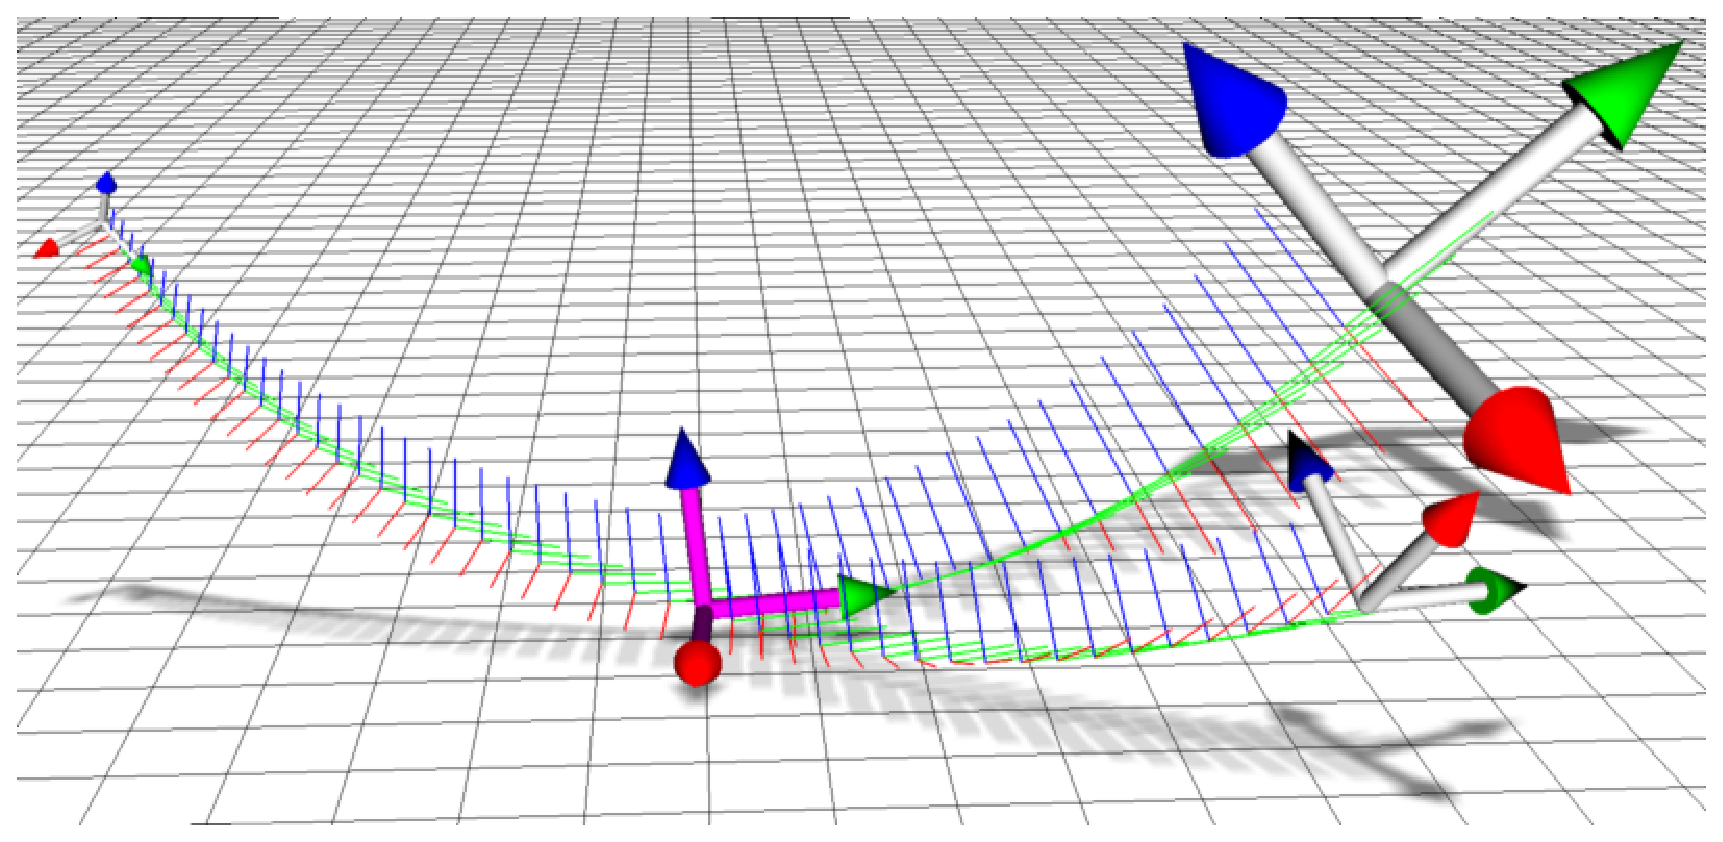
\includegraphics[width=0.95\linewidth]{egfigure.eps}
}

\end{center}
   \caption{\small Example of caption.  It is set in Roman so that mathematics (always set in Roman: $B \sin A = A \sin B$) may be included without an
   ugly clash.}
\label{fig:long}
\label{fig:onecol}
\end{figure}

%=========================================================================
\section{CONCLUSIONS}

The paper ends with a conclusion.



%=========================================================================

\section*{ACKNOWLEDGMENT}

This section should come before the Appendices. Funding information may also be included here. The preferred spelling of the word ``acknowledgment'' in American English is without an ``e'' after the ``g.'' Use the singular heading even if you have many acknowledgments. Avoid expressions such as ``One of us (S.B.A.) would like to thank ... .'' Instead, write ``F. A. Author thanks ... .'' In most cases, sponsor and financial support acknowledgments are placed in the unnumbered footnote on the first page, not here.

%=========================================================================
\section*{APPENDIX}

Appendices should be used only when sophisticated technical details are crucial to be included in the paper.
%=========================================================================

%=========================================================================
% References
% BibTeX users please use
\bibliographystyle{IEEEtran} % sorted IEEE style
%\bibliographystyle{spmpsci_unsort}
\bibliography{template.bib} % name your BibTeX database
\hfill {\it Received on October 14, 2003}

\hfill {\it Accepted on January 14, 2004}
\end{document}
